\chapter{Diseño}
\title{Diseño}
\label{cap:Diseno}

\section{Arquitectura}
Como se ha ido viendo en los capítulos anteriores, el dispositivo que se desea desarrollar
tiene que hacer la función básica del director de la banda de música durante una actuación,
es decir, marcar el mismo pulso a los músicos.\\

Si recordamos el esquema planteado en la figura \ref{fig:modeladoconceptual} y todo lo
que se ha ido desarrollando a través de los capítulos anteriores, podemos decir
que el sistema sigue una arquitectura de repositorio -o pizarra- (siendo el repositorio activo):

\begin{itemize}
  \item El director es el centro de todo. Se encarga de realizar la comunicación con los músicos
  \item Los músicos son subsistemas independientes (aunque tengan que estar sincronizados)
  \item Alto acoplamiento entre los músicos y el director
\end{itemize}

A parte de la relación existente entre músicos y director, no debemos olvidar que
deseamos comunicarnos desde un dispositivo (Android según las especificaciones pero que,
como se verá en la implementación, valdrá cualquier SO). Es por ello que el diagrama
de despliegue queda como en la figura \ref{fig:diagramadespliegue}.\\


\begin{figure}[htb]
\centering
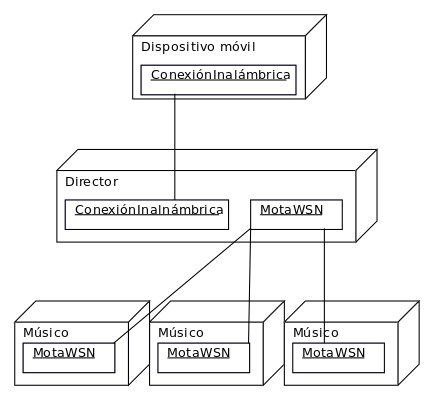
\includegraphics[width=1\textwidth]{./imagenes/diagramadespliegue}
\caption{Diagrama de despliegue} \label{fig:diagramadespliegue}
\end{figure}

\section{Diagramas de comunicación}
\title{Diagramas de comunicación}

Los casos de uso expuestos en \ref{subsec:casosdeuso} se han sideñado según
se muestra en las figuras \ref{fig:comunicacion1},  \ref{fig:comunicacion2} y
\ref{fig:comunicacion3}.\\

\begin{figure}[htb]
\centering
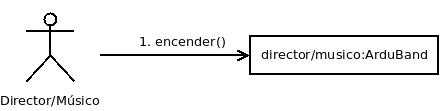
\includegraphics[width=1\textwidth]{./imagenes/comunicacion1}
\caption{Diagrama de comunicación 1} \label{fig:comunicacion1}
\end{figure}

\begin{figure}[htb]
\centering
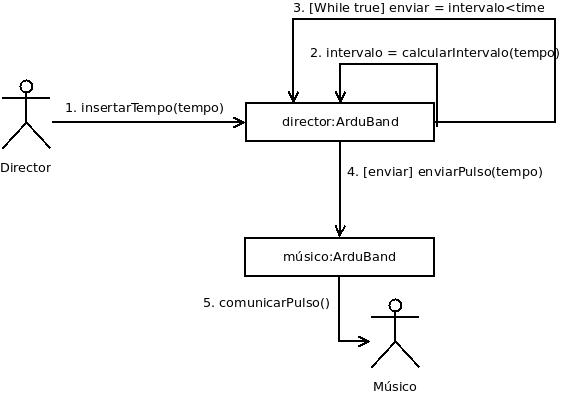
\includegraphics[width=1\textwidth]{./imagenes/comunicacion2}
\caption{Diagrama de comunicación 2} \label{fig:comunicacion2}
\end{figure}

\begin{figure}[htb]
\centering
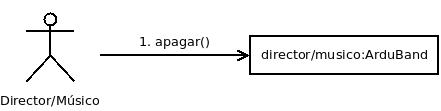
\includegraphics[width=1\textwidth]{./imagenes/comunicacion3}
\caption{Diagrama de comunicación 3} \label{fig:comunicacion3}
\end{figure}
